\subsection{Room identifiers}
\label{sec:application:building_the_model:room_identifiers}

In the fifth step, the room identifiers are introduced by introducing another $\type{string}$ field. This step introduces gives each room a size, or in model terms, the $\type{room\_size}$ attribute on the $.\type{Room}$ class is introduced, including its values. \cref{subsec:library_of_transformations:type_level_transformations:enum_fields} is used to introduce the field on the type level, while on the instance level, \cref{subsec:library_of_transformations:instance_level_transformations:enum_field_values} is used to introduce the values.

The $classtype$ of the new field is $.\type{Room}$, as the field will be defined for rooms. The $name$ of the new field is $\type{room\_\!id}$ and the $fieldtype$ is $.\type{string}$. The set of objects of which the value is set is equal to all room objects, so $objects = \{TRRoom1, TRRoom2, BHPRoomA, BHPRoomB, BHPRoomC\}$. The function for $obids$ returns the existing identifier of each of these objects. The $values$ function is defined as follows:
\begin{align*}
    values = \{&(TRRoom1, \text{``1''}), (TRRoom2, \text{``2''}), (BHPRoomA, \text{``A''}), \\&(BHPRoomB, \text{``B''}), (BHPRoomC, \text{``C''})\}
\end{align*}

The following model is obtained:

\LTXtable{\textwidth}{tex/06_application/02_building_the_model/tables/05_room_identifiers.tex}

\begin{figure}[p]
    \centering
    \begin{subfigure}{0.98\textwidth}
        \centering
        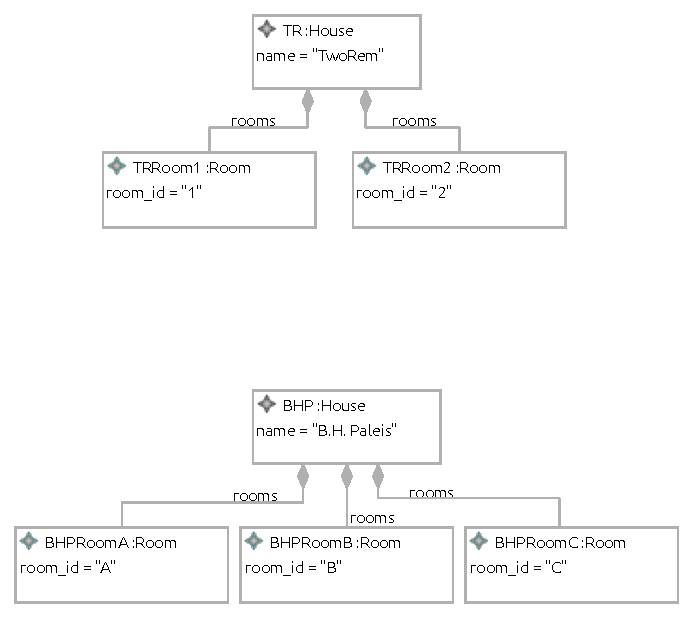
\includegraphics{images/06_application/instance_model/step05.pdf}
        \caption{Instance Model $Im_5$}
        \label{fig:application:building_the_model:room_identifiers:ecore:instance_model}
    \end{subfigure}
    \\
    \begin{subfigure}{0.98\textwidth}
        \centering
        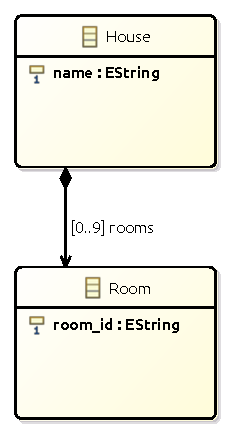
\includegraphics{images/06_application/type_model/step05.pdf}
        \caption{Type Model $Tm_5$}
        \label{fig:application:building_the_model:room_identifiers:ecore:type_model}
    \end{subfigure}
    \caption{The Ecore model after step 5}
    \label{fig:application:building_the_model:room_identifiers:ecore}
\end{figure}

\begin{figure}[p]
    \centering
    \begin{subfigure}{0.98\textwidth}
        \centering
        % To use this figure in your LaTeX document
% import the package groove/resources/groove2tikz.sty
%
\begin{tikzpicture}[scale=\tikzscale,name prefix=step05-]
\node[type_node] (n0) at (0.740, -0.400) {\ml{\textbf{House}\\name: \textbf{string}}};
\node[type_node] (n1) at (0.730, -1.585) {\ml{\textbf{Room}\\room\_id: \textbf{string}}};

\path[basic_edge, composite](n0.south -| 0.730, -1.585) -- node[lab] {\ml{rooms}} (n1) ;
\end{tikzpicture}

        \caption{Instance Graph $IG_5$}
        \label{fig:application:building_the_model:room_identifiers:groove:instance_graph}
    \end{subfigure}
    \\
    \begin{subfigure}{0.98\textwidth}
        \centering
        % To use this figure in your LaTeX document
% import the package groove/resources/groove2tikz.sty
%
\begin{tikzpicture}[scale=\tikzscale,name prefix=step05-]
\node[type_node] (n0) at (0.740, -0.400) {\ml{\textbf{House}\\name: \textbf{string}}};
\node[type_node] (n1) at (0.730, -1.585) {\ml{\textbf{Room}\\room\_id: \textbf{string}}};

\path[basic_edge, composite](n0.south -| 0.730, -1.585) -- node[lab] {\ml{rooms}} (n1) ;
\end{tikzpicture}

        \caption{Type Graph $TG_5$}
        \label{fig:application:building_the_model:room_identifiers:groove:type_graph}
    \end{subfigure}
    \caption{The GROOVE graphs after step 5}
    \label{fig:application:building_the_model:room_identifiers:groove}
\end{figure}

A visual representation of $Tm_5$ and $Im_5$ can be found in \cref{fig:application:building_the_model:room_identifiers:ecore}. Similarly, a visual representation of $TG_5$ and $IG_5$ can be found in \cref{fig:application:building_the_model:room_identifiers:groove}. Please note that because of the definitions of $f_5(Im_5)$ and $f'_5(IG_5)$, we have that $f_5(Im_5) = IG_5$ and $f'_5(IG_5) = Im_5$. Furthermore, $f_5(Im_5)$ and $f'_5(IG_5)$ are valid mapping functions themselves, such that they can be combined with another mapping function in the next step.

The visualisation unveils no surprising details. A string field was already added earlier to the house objects and introducing such a field on the room only shows that it is indeed possible to introduce fields on contained objects.

\afterpage{\FloatBarrier}